% ============================================================
%  Luận văn tốt nghiệp — Bài trình bày bảo vệ
%  Sinh viên : Nguyễn Trương Minh Hoàng (MSSV 2270757)
%  GVHD      : TS. Lê Trọng Nhân
%  Trường    : Trường ĐH Bách Khoa TP.HCM
% ============================================================
\documentclass[aspectratio=169,12pt]{beamer}

% ---------- Encoding & Language ----------
\usepackage[utf8]{inputenc}
\usepackage[T5]{fontenc}
\usepackage[vietnamese]{babel}

% ---------- Fonts & Math ----------
\usepackage{lmodern}
\usepackage{amsmath,amssymb}

% ---------- Theme ----------
\usetheme{Madrid}
\usecolortheme{default}
\setbeamertemplate{navigation symbols}{}
\setbeamertemplate{footline}{
  \leavevmode
  \hbox{%
    \begin{beamercolorbox}[wd=.45\paperwidth,ht=2.5ex,dp=1.5ex,leftskip=2ex]{author in head/foot}%
      \usebeamerfont{author in head/foot}\insertshortauthor
    \end{beamercolorbox}%
    \begin{beamercolorbox}[wd=.45\paperwidth,ht=2.5ex,dp=1.5ex,center]{title in head/foot}%
      \usebeamerfont{title in head/foot}\insertshorttitle
    \end{beamercolorbox}%
    \begin{beamercolorbox}[wd=.10\paperwidth,ht=2.5ex,dp=1.5ex,rightskip=2ex,right]{date in head/foot}%
      \insertframenumber{} / \inserttotalframenumber
    \end{beamercolorbox}}%
  \vskip0pt%
}
\setbeamercolor{frametitle}{bg=blue!70!black, fg=white}
\setbeamercolor{block title}{bg=blue!60!black, fg=white}
\setbeamercolor{block body}{bg=blue!5}

% ---------- Tables & Graphics ----------
\usepackage{booktabs}
\usepackage{multirow}
\usepackage{makecell}
\usepackage{graphicx}
\usepackage{xcolor}
\usepackage{tikz}
\usetikzlibrary{arrows.meta, positioning, shapes.geometric, fit}

% ---------- Utilities ----------
\usepackage{array}
\usepackage{setspace}
% Symbols (use pifont for ding symbols to avoid amssymb conflict)
\usepackage{pifont}
\newcommand{\cmark}{\textcolor{green!60!black}{\ding{51}}}
\newcommand{\xmark}{\textcolor{red!70!black}{\ding{55}}}

% ============================================================
%  Meta
% ============================================================
\title[Framework Tạo Mô hình AI cho HAR]{%
  Xây dựng Framework Tạo Mô hình AI\\
  cho Ứng dụng Theo dõi Chuyển động Con người}
\subtitle{Luận văn tốt nghiệp --- Bảo vệ luận văn}
\author[Nguyễn Trương Minh Hoàng]{%
  \textbf{Sinh viên:} Nguyễn Trương Minh Hoàng (MSSV 2270757)\\[2pt]
  \textbf{GVHD:} TS. Lê Trọng Nhân}
\institute[HCMUT]{%
  Khoa Khoa học \& Kỹ thuật Máy tính\\
  Trường Đại học Bách Khoa TP.HCM}
\date{Tháng 6 năm 2026}

% ============================================================
\begin{document}

% ----------------------------------------------------------
% SLIDE 1 — Trang bìa
% ----------------------------------------------------------
\begin{frame}
  \titlepage
\end{frame}

% ----------------------------------------------------------
% SLIDE 2 — Nội dung trình bày
% ----------------------------------------------------------
\begin{frame}{Nội dung trình bày}
  \begin{enumerate}
    \item Bối cảnh, bài toán và mục tiêu nghiên cứu
    \item Framework đề xuất và quy trình hoạt động
    \item Thiết lập thực nghiệm và kết quả chính
    \item Kết quả triển khai thiết bị và so sánh nền tảng
    \item Kết luận, giới hạn và hướng phát triển
  \end{enumerate}
  \vspace{6pt}
  \small\textit{Mục tiêu trình bày 20 phút: tập trung vào bài toán, giải pháp, bằng chứng thực nghiệm và giá trị thực tiễn của framework.}
\end{frame}

\section{Bối cảnh}
\section{Mục tiêu}
\section{Framework đề xuất}
\section{Thực nghiệm}
\section{Kết luận}

% ===========================================================
%  PHẦN 1 — BỐI CẢNH & VẤN ĐỀ
% ===========================================================

% Gợi ý nói (1.5 phút): Mở đầu từ nhu cầu HAR trên thiết bị đeo, sau đó dẫn sang khoảng trống giữa mô hình Python và triển khai thực tế trên MCU.
\begin{frame}{Bối cảnh \& Bài toán}
  \begin{columns}[T]
    \column{0.52\textwidth}
      \textbf{HAR dựa trên IMU} có nhu cầu cao trong:
      \begin{itemize}
        \item \textbf{Y tế:} phát hiện té ngã, phục hồi chức năng
        \item \textbf{Thể thao:} phân tích kỹ thuật, đếm bài tập
        \item \textbf{Công nghiệp:} phát hiện tư thế nguy hiểm
      \end{itemize}
      \vspace{6pt}
      \textbf{Yêu cầu triển khai thực tế:}
      \begin{itemize}
        \item suy luận trực tiếp trên thiết bị biên
        \item độ trễ thấp, tiết kiệm năng lượng
        \item không phụ thuộc kết nối mạng
      \end{itemize}

    \column{0.46\textwidth}
      \begin{block}{Khoảng trống nghiên cứu}
        \centering\small
        \begin{tikzpicture}[
          node distance=0.32cm,
          box/.style={rectangle, rounded corners=2pt, draw=blue!60, fill=blue!8,
                      minimum width=2.6cm, minimum height=0.55cm,
                      align=center, font=\scriptsize},
          arr/.style={-{Stealth[length=4pt]}, thick, blue!60}]
          \node[box] (raw)   {Dữ liệu IMU thô};
          \node[box, below=of raw]  (pre)  {Tiền xử lý / Lọc};
          \node[box, below=of pre]  (seg)  {Phân đoạn cửa sổ};
          \node[box, below=of seg]  (feat) {Trích xuất đặc trưng};
          \node[box, below=of feat] (ml)   {Huấn luyện ML};
          \node[box, below=of ml]   (dep)  {Triển khai thiết bị};
          \draw[arr] (raw)--(pre); \draw[arr] (pre)--(seg);
          \draw[arr] (seg)--(feat); \draw[arr] (feat)--(ml);
          \draw[arr] (ml)--(dep);
        \end{tikzpicture}
      \end{block}
      \vspace{4pt}
      \small Phần lớn công trình dừng ở bước huấn luyện ngoại tuyến; phần triển khai trên MCU còn rời rạc, khó kiểm chứng và khó tái sử dụng.
  \end{columns}
\end{frame}

% Gợi ý nói (1 phút): Nói rõ mục tiêu luận văn là framework, không phải chỉ tối ưu một mô hình HAR riêng lẻ.
\begin{frame}{Mục tiêu nghiên cứu \& Câu hỏi chính}
  \begin{block}{Câu hỏi trung tâm}
    Có thể xây dựng một framework mã nguồn mở giúp người dùng đi từ dữ liệu IMU thô đến mã suy luận chạy trên vi điều khiển một cách nhất quán, minh bạch và tái sử dụng được hay không?
  \end{block}

  \vspace{6pt}
  \begin{columns}[T]
    \column{0.50\textwidth}
      \textbf{Mục tiêu:}
      \begin{itemize}\small
        \item Tạo pipeline end-to-end cho HAR trên IMU
        \item Giảm rào cản kỹ thuật ở bước tiền xử lý và triển khai
        \item Đảm bảo tính tương đồng giữa huấn luyện và suy luận thiết bị
        \item Hỗ trợ nhiều mô hình và nhiều đích triển khai
      \end{itemize}

    \column{0.50\textwidth}
      \textbf{Phạm vi đánh giá:}
      \begin{itemize}\small
        \item Dữ liệu IMU 6 trục, 100 Hz
        \item 5 hoạt động người dùng
        \item RF, SVM, NN, PyTorch MLP, CNN
        \item Thiết bị tham chiếu: Seeed XIAO nRF52840 Sense
      \end{itemize}
  \end{columns}
\end{frame}

% ===========================================================
%  PHẦN 2 — MỤC TIÊU & ĐÓNG GÓP
% ===========================================================

% Gợi ý nói (1 phút): Chọn 4–5 ý thật rõ. Nhấn mạnh giá trị của framework thay vì kể chi tiết lỗi kỹ thuật.
\begin{frame}{Đóng góp chính của luận văn}
  \begin{columns}[T]
    \column{0.5\textwidth}
      \textbf{Về hệ thống:}
      \begin{itemize}\small
        \item \cmark\ Framework end-to-end: dữ liệu $\rightarrow$ đặc trưng $\rightarrow$ huấn luyện $\rightarrow$ mã triển khai
        \item \cmark\ Giao diện kéo thả cho tiền xử lý và phân đoạn cửa sổ
        \item \cmark\ Lưu trữ artifact huấn luyện theo dạng dùng lại được
      \end{itemize}

    \column{0.5\textwidth}
      \textbf{Về triển khai:}
      \begin{itemize}\small
        \item \cmark\ Bảo đảm parity Python\,$\leftrightarrow$\,C++ trong pipeline trích xuất đặc trưng
        \item \cmark\ Hỗ trợ RF, SVM, NN, PyTorch MLP và CNN
        \item \cmark\ Sinh mã cho Arduino-compatible, ARM Cortex-M, Zephyr, MicroPython
        \item \cmark\ Xác thực bằng kết quả huấn luyện và thử nghiệm trên thiết bị thực
      \end{itemize}
  \end{columns}
\end{frame}

% ===========================================================
%  PHẦN 3 — KIẾN TRÚC FRAMEWORK
% ===========================================================

% Gợi ý nói (1.5 phút): Đây là slide xương sống. Đi đúng thứ tự trái sang phải và chốt rằng mọi tab dùng cùng một pipeline thống nhất.
\begin{frame}{Kiến trúc Framework}
  \begin{center}
  \begin{tikzpicture}[
    tab/.style={rectangle, rounded corners=3pt, draw=blue!70, fill=blue!12,
                minimum width=1.55cm, minimum height=1.1cm,
                align=center, font=\scriptsize\bfseries},
    arr/.style={-{Stealth[length=5pt]}, thick, blue!60},
    lbl/.style={font=\tiny, text=gray!80, align=center}]

    \node[tab] (d1) {Dữ liệu\\(Tab 1)};
    \node[tab, right=0.55cm of d1] (d2) {Tiền xử lý\\(Tab 2)};
    \node[tab, right=0.55cm of d2] (d3) {Đặc trưng\\(Tab 3)};
    \node[tab, right=0.55cm of d3] (d4) {Huấn luyện\\(Tab 4)};
    \node[tab, right=0.55cm of d4] (d5) {Tạo mã\\(Tab 5)};
    \node[tab, right=0.55cm of d5] (d6) {Kiểm tra\\(Tab 6)};

    \draw[arr] (d1)--(d2); \draw[arr] (d2)--(d3);
    \draw[arr] (d3)--(d4); \draw[arr] (d4)--(d5);
    \draw[arr] (d5)--(d6);

    \node[lbl, below=0.18cm of d1] {CSV\\100\,Hz};
    \node[lbl, below=0.18cm of d2] {Lọc\\Kéo thả};
    \node[lbl, below=0.18cm of d3] {63\,feat\\6 chế độ};
    \node[lbl, below=0.18cm of d4] {RF/SVM\\NN/CNN};
    \node[lbl, below=0.18cm of d5] {C++/MPy\\4 platform};
    \node[lbl, below=0.18cm of d6] {Serial\\XIAO};
  \end{tikzpicture}
  \end{center}

  \vspace{4pt}
  \begin{columns}[T]
    \column{0.32\textwidth}
      \begin{block}{\small Công nghệ}
        \scriptsize
        Python 3 · Dash 2.14\\
        scikit-learn · PyTorch\\
        joblib · pandas · numpy
      \end{block}
    \column{0.34\textwidth}
      \begin{block}{\small Lưu trữ trạng thái}
        \scriptsize
        \texttt{persistent\_data/}\\
        CSV $\to$ joblib $\to$ .h/.ino\\
        Không cần database
      \end{block}
    \column{0.32\textwidth}
      \begin{block}{\small Thiết bị tham chiếu}
        \scriptsize
        Seeed XIAO nRF52840\\
        IMU LSM6DS3, 6 trục\\
        ARM Cortex-M4F 64\,MHz
      \end{block}
  \end{columns}
\end{frame}

% Gợi ý nói (1.5 phút): Giải thích nhanh dữ liệu, thiết bị, bài toán 3 lớp và 5 lớp, rồi nói đây là nền cho mọi kết quả sau.
\begin{frame}{Thiết lập thực nghiệm}
  \begin{columns}[T]
    \column{0.52\textwidth}
      \textbf{Dữ liệu và phần cứng:}
      \begin{itemize}\small
        \item IMU 6 trục, 100 Hz, thiết bị Seeed XIAO nRF52840 Sense
        \item 5 hoạt động: running, still, walking, walking downstairs, walking upstairs
        \item 2 cấu hình đánh giá: bài toán 3 lớp và 5 lớp
      \end{itemize}

      \textbf{Cấu hình xử lý:}
      \begin{itemize}\small
        \item Cửa sổ 150 mẫu (1,5 s), bước trượt 75 mẫu
        \item Đặc trưng mặc định: \texttt{orientation\_invariant} (63 đặc trưng)
        \item CNN dùng trực tiếp đầu vào thô $150 \times 6$
        \item Chia dữ liệu: train / validation / test
      \end{itemize}

    \column{0.46\textwidth}
      \begin{center}
        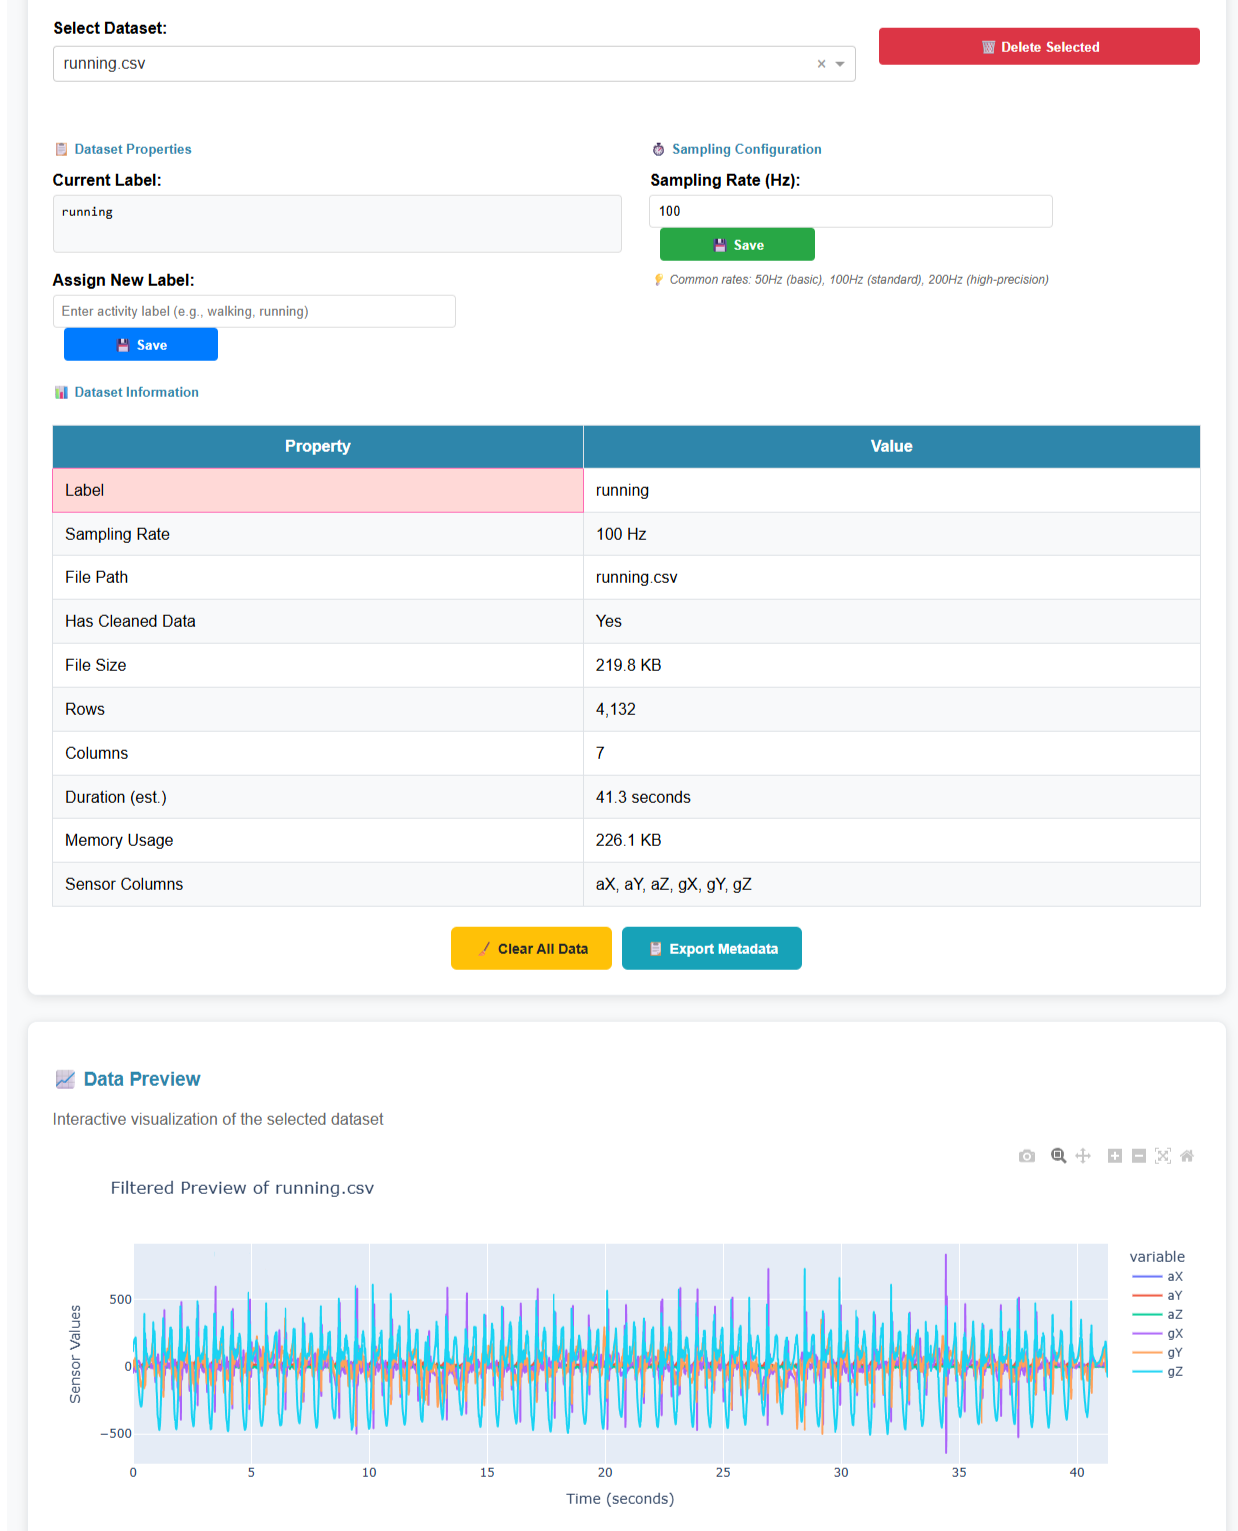
\includegraphics[width=\linewidth, height=4.6cm, keepaspectratio]{figures/ui_data_upload.png}\\
        \vspace{4pt}
        \scriptsize\textit{Giao diện quản lý dữ liệu đầu vào của framework}
      \end{center}
  \end{columns}
\end{frame}

% Gợi ý nói (2 phút): Đây là chỗ nói giá trị “dễ dùng nhưng vẫn kiểm soát được”. Không đi quá sâu công thức; chỉ nói những quyết định thiết kế chính.
\begin{frame}{Tiền xử lý \& Trích xuất đặc trưng}
  \begin{columns}[T]
    \column{0.5\textwidth}
      \textbf{Tiền xử lý tương tác:}
      \begin{itemize}\small
        \item Kéo thả trực tiếp vùng hoạt động trên biểu đồ tín hiệu
        \item Hỗ trợ các bộ lọc Butterworth, Savitzky-Golay, Kalman
        \item Đệm cửa sổ bằng lặp giá trị biên để giữ tính hợp lý vật lý
      \end{itemize}
      \vspace{4pt}
      \textbf{Trích xuất đặc trưng:}
      \begin{itemize}\small
        \item 6 chế độ đặc trưng phục vụ nhiều mức tài nguyên khác nhau
        \item Chế độ mặc định: \texttt{orientation\_invariant}
        \item 15 thống kê/tín hiệu: mean, std, min, max, median, IQR, RMS, energy, ...
      \end{itemize}

    \column{0.5\textwidth}
      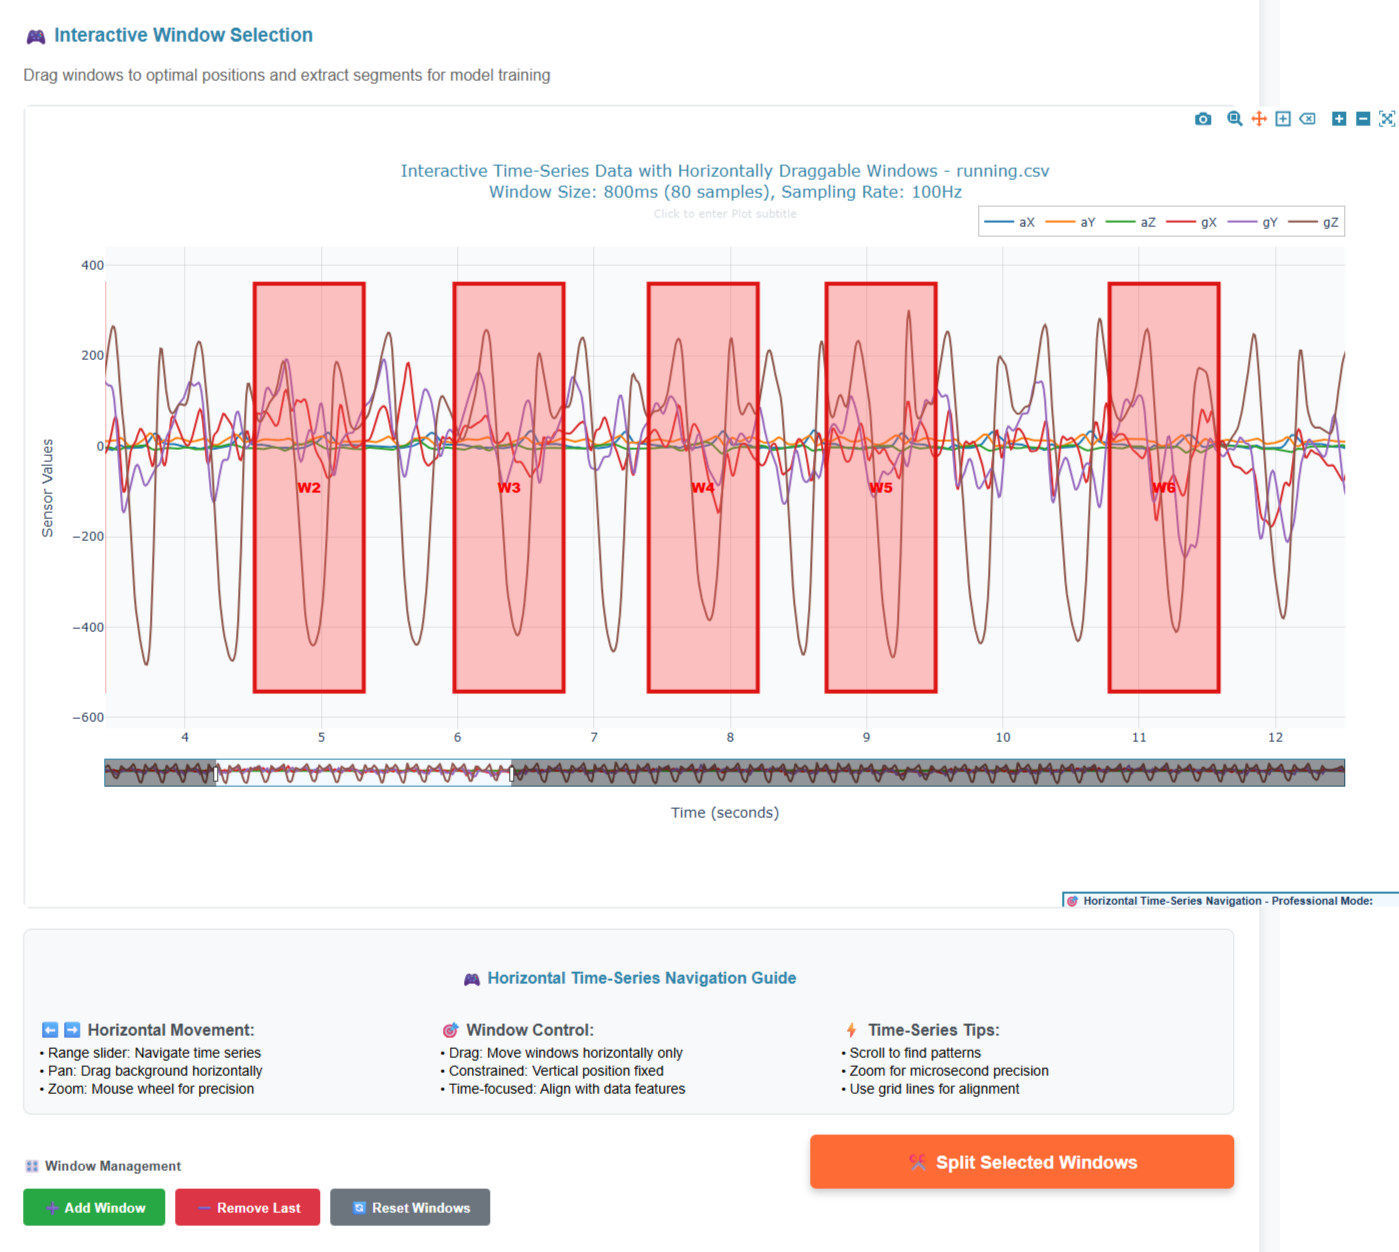
\includegraphics[width=\linewidth, height=4.3cm, keepaspectratio]{figures/ui_preprocessing_draggable.png}\\
      \vspace{4pt}
      \scriptsize\textit{Giao diện tiền xử lý và phân đoạn cửa sổ kéo thả}
      \vspace{6pt}

      \small\textbf{Thông điệp chính:} framework cho phép người dùng kiểm soát trực tiếp bước tiền xử lý thay vì xem đó là một hộp đen.
  \end{columns}
\end{frame}

% Gợi ý nói (1.5 phút): Nêu 3 ý: nhiều mô hình, nhiều nền tảng, cùng một model artifact được tái sử dụng để sinh mã.
\begin{frame}{Huấn luyện mô hình \& Tạo mã triển khai}
  \begin{columns}[T]
    \column{0.48\textwidth}
      \textbf{Các mô hình được hỗ trợ:}
      \begin{itemize}\small
        \item Random Forest
        \item SVM (RBF)
        \item Neural Network (scikit-learn)
        \item PyTorch MLP
        \item PyTorch CNN
      \end{itemize}

      \vspace{6pt}
      \textbf{Ý tưởng triển khai:}
      \begin{itemize}\small
        \item Model sau huấn luyện được lưu thành artifact thống nhất
        \item Từ artifact này, framework sinh mã cho nhiều nền tảng khác nhau
        \item Người dùng không cần viết tay phần suy luận trên MCU
      \end{itemize}

    \column{0.52\textwidth}
      \textbf{Nền tảng đích được hỗ trợ:}
      \begin{itemize}\small
        \item Arduino-compatible (XIAO, ESP32, M5Stack, Teensy)
        \item ARM Cortex-M generic (C không phụ thuộc thư viện)
        \item ESP-IDF, Zephyr RTOS
        \item MicroPython (không cần NumPy)
        \item TFLite Micro / ONNX Runtime (NN/CNN)
      \end{itemize}
      \vspace{4pt}
      \textbf{4 chế độ tối ưu:}
      \begin{itemize}\small
        \item \texttt{accuracy}: 6 chữ số thập phân, debug bật
        \item \texttt{balanced}: 3 chữ số (mặc định)
        \item \texttt{speed}: 2--3 chữ số, tối ưu bộ đệm
        \item \texttt{power}: 3--4 chữ số, tối ưu năng lượng
      \end{itemize}
      \vspace{4pt}
      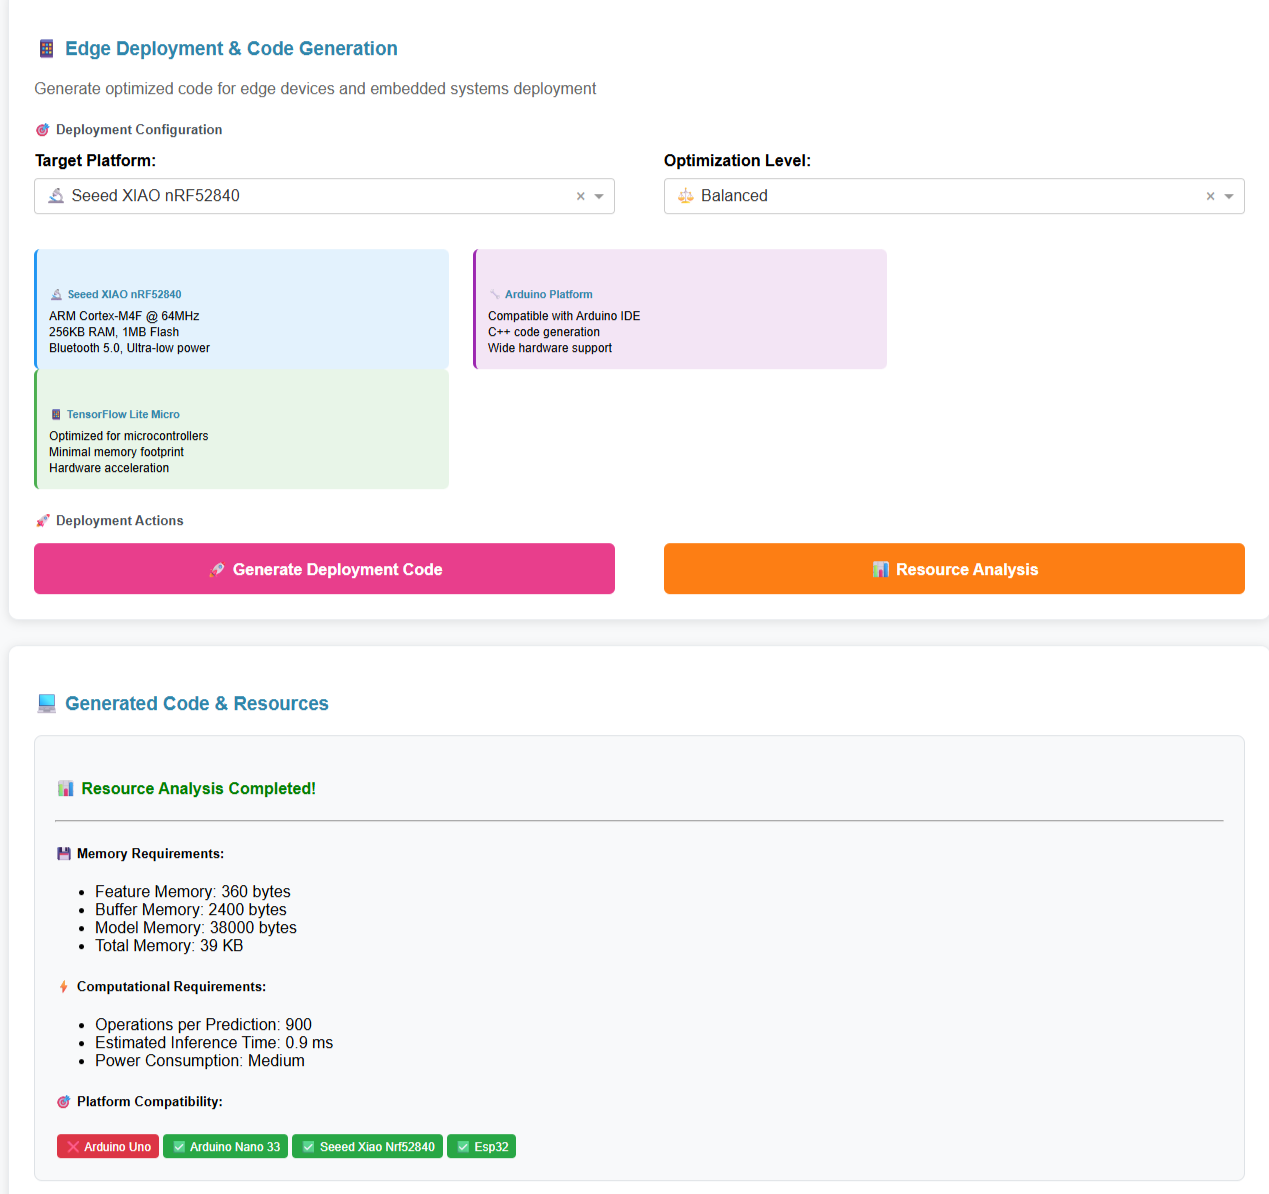
\includegraphics[width=\linewidth, height=2.5cm, keepaspectratio]{figures/ui_code_generation.png}
  \end{columns}
\end{frame}

% ===========================================================
%  PHẦN 5 — KẾT QUẢ THỰC NGHIỆM
% ===========================================================

% Gợi ý nói (2.5 phút): Đây là slide bằng chứng chính. Nói nhanh kết quả 3 lớp, tập trung vào 5 lớp vì khó hơn và có giá trị hơn.
\begin{frame}{Kết quả Thực nghiệm}
  \textbf{Thiết lập chính:} IMU 6 trục, 100\,Hz, cửa sổ 150 mẫu, bước 75, đặc trưng \texttt{orientation\_invariant}.

  \vspace{4pt}
  \begin{columns}[T]
    \column{0.48\textwidth}
      \centering\small\textbf{Bài toán 5 lớp} (229 mẫu kiểm tra)
      \begin{tabular}{@{}lcc@{}}
        \toprule
        Thuật toán & Acc. (\%) & F1 \\
        \midrule
        PyTorch MLP & \textbf{99,13} & 0,990 \\
        PyTorch 1D-CNN & \textbf{99,13} & 0,992 \\
        Neural Network & 98,69 & 0,984 \\
        Random Forest & 98,25 & 0,981 \\
        SVM (RBF) & 97,38 & 0,972 \\
        \bottomrule
      \end{tabular}
      \vspace{4pt}\\
      \scriptsize\textbf{Nhận xét:} chênh lệch giữa mô hình tốt nhất và thấp nhất chỉ 1,75 điểm \%, cho thấy pipeline đặc trưng có chất lượng tốt.

    \column{0.52\textwidth}
      \centering
      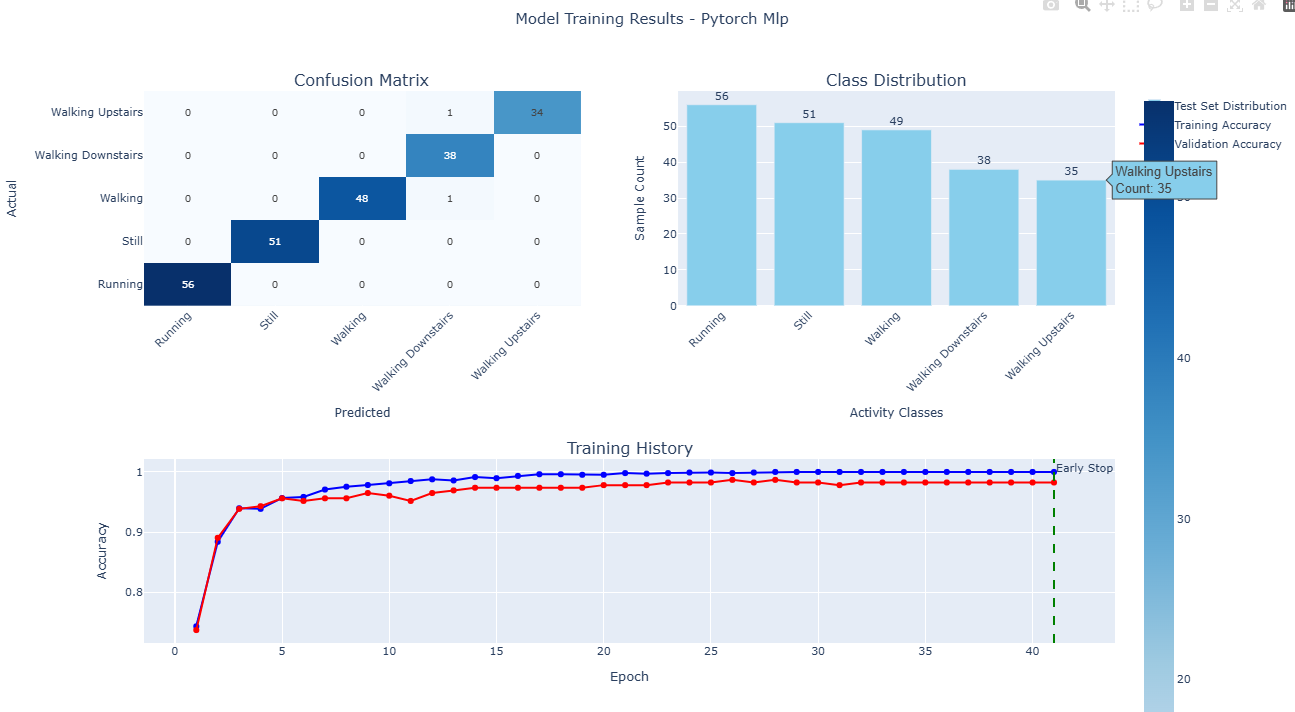
\includegraphics[width=\linewidth, height=4.5cm, keepaspectratio]{figures/ui_mlp_training_c5_confusion.png}\\
      \vspace{4pt}
      \scriptsize Ma trận nhầm lẫn của PyTorch MLP: lỗi chủ yếu xuất hiện giữa các lớp đi bộ và cầu thang.
  \end{columns}
  \vspace{4pt}
  \small\textbf{Ghi chú ngắn:} bài toán 3 lớp đạt 100\% trên cả 5 thuật toán, chứng tỏ framework hoạt động tốt ngay cả với các cấu hình đơn giản hơn.
\end{frame}

% Gợi ý nói (2 phút): Chuyển từ kết quả offline sang giá trị triển khai. Đây là nơi nhấn mạnh thesis không dừng ở training accuracy.
\begin{frame}{Kết quả Triển khai Thiết bị (Seeed XIAO nRF52840)}
  \begin{columns}[T]
    \column{0.52\textwidth}
      \textbf{Kết quả triển khai:}
      \begin{itemize}\small
        \item PyTorch 1D-CNN: \textbf{ổn định cả 3 và 5 lớp}
        \item NN sklearn: lỗi phân loại running trong một số điều kiện
        \item Random Forest: ổn định cho 3 lớp
        \item Ngưỡng confidence: loại bỏ dự đoán không chắc chắn
      \end{itemize}

      \vspace{6pt}
      \textbf{Yêu cầu tài nguyên (Neural Network 5 lớp):}
      \begin{itemize}\small
        \item Flash: $\sim$95\,KB (bao gồm trọng số + FE + scaler)
        \item SRAM: $<$8\,KB (bộ đệm cửa sổ + tính toán)
        \item Thời gian suy luận: $<$100\,ms tại 64\,MHz
      \end{itemize}
      \vspace{4pt}
      \small Ý nghĩa: framework không chỉ tạo mô hình tốt trên máy tính mà còn tạo artifact dùng được trên thiết bị biên thật.

    \column{0.47\textwidth}
      \begin{block}{So sánh với TFLite Micro}
        \small
        \begin{tabular}{@{}lcc@{}}
          \toprule
          & Framework & TFLite \\
          \midrule
          Flash (NN) & 95\,KB & $\sim$245\,KB \\
          RF hỗ trợ & \cmark & \xmark \\
          SVM hỗ trợ & \cmark & \xmark \\
          Mã có thể đọc & \cmark & \xmark \\
          \bottomrule
        \end{tabular}
      \end{block}

      \vspace{6pt}
      \begin{alertblock}{\small Thông điệp chính}
        \scriptsize
        Độ chính xác ngoại tuyến là cần thiết nhưng chưa đủ; giá trị thực của framework nằm ở khả năng đưa mô hình ra thiết bị với quy trình có thể kiểm tra và tái sử dụng.
      \end{alertblock}
  \end{columns}
\end{frame}

% ===========================================================
%  PHẦN 6 — SO SÁNH NỀN TẢNG THƯƠNG MẠI
% ===========================================================

% Gợi ý nói (2 phút): Chỉ so sánh ở mức thesis cần chứng minh: minh bạch, chi phí, phạm vi mô hình, khả năng triển khai.
\begin{frame}{So sánh với Nền tảng Thương mại}
  \begin{center}
  \scriptsize
  \setlength{\tabcolsep}{4pt}
  \begin{tabular}{@{}p{3.4cm}p{2.0cm}p{2.0cm}p{2.4cm}@{}}
    \toprule
    \textbf{Tiêu chí} & \textbf{Edge Impulse} & \textbf{SensiML} & \textbf{Framework này} \\
    \midrule
    Chi phí & \$20--99/tháng & \$99--500/tháng & Miễn phí \\
    Mã nguồn mở & \xmark & \xmark & \cmark \\
    Minh bạch pipeline triển khai & Hộp đen & Hộp đen & \cmark\ Toàn bộ \\
    Hỗ trợ RF/SVM & Giới hạn & Có chọn lọc & \cmark \\
    Đảm bảo parity & Không rõ & Không rõ & \cmark\ Bit-exact \\
    \midrule
    F1 trên 3 lớp & 0,96 & --- & \textbf{1,00} \\
    Flash (NN) & 51\% & --- & \textbf{18--23\%} \\
    \bottomrule
  \end{tabular}
  \end{center}

  \vspace{2pt}
  \begin{exampleblock}{\small Điểm mạnh độc đáo}
    \small Giá trị khác biệt của framework là \textbf{minh bạch + tái sử dụng + hỗ trợ nhiều mô hình}, thay vì chỉ tối ưu trải nghiệm kéo-thả như các nền tảng thương mại.
  \end{exampleblock}
\end{frame}

% ===========================================================
%  PHẦN 7 — KẾT LUẬN
% ===========================================================

% Gợi ý nói (1.5 phút): Kết luận theo đúng thesis claim: xây được framework, đã kiểm chứng, còn giới hạn dữ liệu và benchmark.
\begin{frame}{Kết luận \& Hướng phát triển}
  \begin{columns}[T]
    \column{0.52\textwidth}
      \textbf{Đã đạt được:}
      \begin{itemize}\small
        \item \cmark\ Framework end-to-end, mã nguồn mở
        \item \cmark\ 97,38--99,13\% (5 lớp), 100\% (3 lớp)
        \item \cmark\ Tương đồng huấn luyện--triển khai được bảo đảm
        \item \cmark\ Triển khai thành công trên XIAO nRF52840
        \item \cmark\ Vượt Edge Impulse: F1 1,00 vs 0,96
      \end{itemize}

    \column{0.48\textwidth}
      \textbf{Giới hạn và hướng phát triển:}
      \begin{itemize}\small
        \item Hiện mới đánh giá sâu trên dữ liệu một đối tượng và thiết bị tham chiếu
        \item Cần mở rộng sang dữ liệu đa người dùng, đa hướng gắn cảm biến
        \item Có thể bổ sung học liên tục, sensor fusion và tối ưu đa mục tiêu
      \end{itemize}
  \end{columns}

  \vspace{4pt}
  \begin{block}{\small Kết luận tổng quát}
    \small Luận văn chứng minh rằng có thể xây dựng một framework HAR mã nguồn mở giúp rút ngắn khoảng cách từ huấn luyện đến triển khai thiết bị biên, đồng thời vẫn giữ được tính minh bạch và khả năng kiểm chứng.
  \end{block}
\end{frame}

% ----------------------------------------------------------
% SLIDE 14 — Cảm ơn / Q&A
% ----------------------------------------------------------
\begin{frame}
  \begin{center}
    \vspace{0.5cm}
    {\LARGE\bfseries Cảm ơn Quý Thầy/Cô \& Hội đồng}

    \vspace{0.8cm}
    \large Xin mời Hội đồng đặt câu hỏi

    \vspace{1.2cm}
    \normalsize
    \begin{tabular}{rl}
      \textbf{Sinh viên:} & Nguyễn Trương Minh Hoàng \\
      \textbf{MSSV:}      & 2270757 \\
      \textbf{GVHD:}      & TS. Lê Trọng Nhân \\
      \textbf{Đề tài:}    & Framework AI cho HAR trên thiết bị biên \\
    \end{tabular}

    \vspace{1.0cm}
    \small\textit{Xin cảm ơn Quý Thầy/Cô và Hội đồng đã lắng nghe.}
  \end{center}
\end{frame}

% ===========================================================
%  BACKUP SLIDES — Câu hỏi hội đồng
% ===========================================================
\appendix

% Gợi ý dùng khi hội đồng hỏi sâu về consistency giữa Python và C++.
\begin{frame}{[Dự phòng] Nhất quán giữa huấn luyện và triển khai}
  \begin{columns}[T]
    \column{0.5\textwidth}
      \textbf{Các nguyên tắc đảm bảo nhất quán:}
      \begin{enumerate}\scriptsize
        \item Cùng công thức đặc trưng ở Python và C++
        \item Cùng thứ tự đặc trưng khi huấn luyện và sinh mã
        \item Cùng tốc độ lấy mẫu, cửa sổ và chuẩn hóa
        \item Artifact mô hình chứa metadata để tái sử dụng khi triển khai
        \item Các mô hình raw-input như CNN có đường triển khai riêng
      \end{enumerate}

    \column{0.5\textwidth}
      \textbf{Ý nghĩa thực tiễn:}\\[4pt]
      Nếu không kiểm soát tính nhất quán, mô hình có thể đạt kết quả tốt trên máy tính nhưng hoạt động không ổn định khi đưa lên MCU.\\[6pt]

      Framework giải quyết điều này bằng cách giữ toàn bộ chuỗi xử lý trong cùng một pipeline có thể đọc, kiểm tra và tái sử dụng.
  \end{columns}
\end{frame}

\begin{frame}{[Dự phòng] Phân tích Ma trận Nhầm lẫn}
  \begin{columns}[T]
    \column{0.55\textwidth}
      \textbf{Bài toán 5 lớp --- PyTorch MLP (F1 = 0,990):}

      \vspace{4pt}
      \small
      \begin{tabular}{@{}lcc@{}}
        \toprule
        Hoạt động & Precision & Recall \\
        \midrule
        Running & 1,000 & 1,000 \\
        Still & 1,000 & 1,000 \\
        Walking & 1,000 & 0,980 \\
        W. Downstairs & 0,950 & 1,000 \\
        W. Upstairs & 1,000 & 0,971 \\
        \midrule
        \textbf{Macro} & \textbf{0,990} & \textbf{0,990} \\
        \bottomrule
      \end{tabular}

    \column{0.45\textwidth}
      \textbf{Nhận xét:}
      \begin{itemize}\small
        \item Running, Still: F1 = 1,000 (đặc trưng biên độ phân biệt rõ)
        \item Lỗi tập trung ở nhóm đi bộ (walking vs stair variants)
        \item 1 mẫu walking bị nhầm → W.Downstairs (precision 0,950)
        \item Orientation-invariant feature giúp phân biệt tốt hơn per-axis feature trước đây
      \end{itemize}
      \vspace{4pt}
      \includegraphics[width=\linewidth, height=3.0cm, keepaspectratio]%
        {figures/ui_mlp_training_c5_confusion.png}
  \end{columns}
\end{frame}

\begin{frame}{[Dự phòng] Câu hỏi thường gặp}
  \textbf{Q: Tại sao không dùng TFLite Micro cho tất cả?}\\
  \textbf{A:} RF/SVM không có đường chuyển đổi sang TFLite (ONNX-ML operators không được onnx2tf hỗ trợ). Framework hỗ trợ cả hai hướng: tạo mã trực tiếp (tất cả mô hình) + TFLite path (chỉ NN/CNN).

  \vspace{8pt}
  \textbf{Q: Dataset chỉ 1 đối tượng có đủ để đánh giá?}\\
  \textbf{A:} Mục tiêu luận văn là \textit{framework}, không phải xây dựng mô hình HAR tổng quát cuối cùng. Dữ liệu hiện tại đủ để chứng minh pipeline hoạt động end-to-end; mở rộng đa đối tượng là bước tiếp theo.

  \vspace{8pt}
  \textbf{Q: Làm sao biết parity được đảm bảo?}\\
  \textbf{A:} Framework có validation script (\texttt{validate\_deployment.py}) để so sánh đặc trưng Python và C++ trên cùng dữ liệu đầu vào, đồng thời lưu metadata mô hình để tái sử dụng nhất quán khi sinh mã.
\end{frame}

\end{document}
